%!TEX root = ../../Heun_Dale_Haney_A_dynamic_approach_to_input_output_modeling.tex
%%%%%%%%%%%%%%%%%%%%% chapter.tex %%%%%%%%%%%%%%%%%%%%%%%%%%%%%%%%%
%
% sample chapter
%
% Use this file as a template for your own input.
%
%%%%%%%%%%%%%%%%%%%%%%%% Springer-Verlag %%%%%%%%%%%%%%%%%%%%%%%%%%
%\motto{Use the template \emph{chapter.tex} to style the various elements of your chapter content.}
\chapter{Material flows}
% use \chaptermark{}
% to alter or adjust the chapter heading in the running head
\chaptermark{Materials}
% Always give a unique label
\label{chap:materials} 

\abstract*{[NEED TO ADD ABSTRACT HERE]}

%% \abstract{Each chapter should be preceded by an abstract (10--15 lines long) that summarizes the content. The abstract will appear \textit{online} at \url{www.SpringerLink.com} and be available with unrestricted access. This allows unregistered users to read the abstract as a teaser for the complete chapter. As a general rule the abstracts will not appear in the printed version of your book unless it is the style of your particular book or that of the series to which your book belongs.\newline\indent
%% Please use the 'starred' version of the new Springer \texttt{abstract} command for typesetting the text of the online abstracts (cf. source file of this chapter template \texttt{abstract}) and include them with the source files of your manuscript. Use the plain \texttt{abstract} command if the abstract is also to appear in the printed version of the book.}

%% Use the template \emph{chapter.tex} together with the Springer document class SVMono (monograph-type books) or SVMult (edited books) to style the various elements of your chapter content in the Springer layout.

In the Introduction, we introduced the idea that economies are like organisms. 
This chapter explores
this idea further by observing the interchange of materials \emph{within}
an economy, as well as exchanges of materials between an economy and 
surrounding environment---the biosphere. 

% Just as a living organism takes
% in food, water and air, so too an
% economy must take in raw materials from its environment. To a large extent,
% the major exchanges of materials between industrial economies and their 
% environment mirror those of an animal. Large inputs of fresh water, hydrocarbons
% and oxygen with the emission of carbon dioxide and polluted water [REF BRANDT]
% dioxide and hydro-carbons These
% materials are then used for a number of different purposes. Some
% become the building blocks from which the physical structures within the 
% economy---buildings, roads, even people---are composed. These materials
% must be extracted from the environment and processed, transported and then
% manufactured into final goods. Such activities require energy resources. In
% an economy primarily dependent on the combustion of fossil fuels, energy conversion
% of energy necessarily requires the presence of oxygen in the atmosphere and
% the emission of carbon dioxide. Many processes also require flows of materials, 
% especially fresh water, that are not directly embodied in the final product.
 

There are many easily observable instances of material flow within an
economy. I look around my office at my computer screen and coffee cup
and myriad other items. I look out my window to the street and building
opposite. All of these goods came originally from natural resources, be it paper or
petroleum or rock. They were extracted and processed, transported and
transformed requiring yet more materials and energy inputs in the form of
electricity or fuels. 

There are also inumerable material flows caused by an economy that we do not observe.
The extraction of raw materials generates additional overburden---earth that must be
extracted and processed and ultimately discarded without ever entering the economy
proper. Other flows occur around us unseen. The cars outside my window suck in nitrogen
and oxygen (without which the engine would not work) and emit water, carbon dioxide and
other more harmful substances. 

Even services which we tend to think of as non-material, require at least some material
infrastructure. The hairdresser requires scissors (and to a greater or lesser extent 
some hair) with which to work. Even the internet, often lauded as the exemplar of
dematerialization of the economic process, requires a whole host of computer
infrastructure including electricity, data servers, telephone networks and a
computer by which to access it.

In this chapter, we will define a mathematical framework by which to track the flow of
materials within an economy, building from a one-sector economy up to examples of both a
two- and three-sector economy. We will finally apply this framework to the illustrative
example of the US automobile industry that runs through the whole book. First let us
outline the basic methodology.

\section{Methodology}
\label{sec:Materials_Methodology}

% Everyone is familiar with the notion of accounting of material (and even non-material)
% things. In order to be rigorous, the first step requires the definition of what we
% will be counting as well as the place (defined in both time and space) for which we will
% be counting. Engineers often call this a \emph{control volume}. For example, I may wish
% to account the number of apples in my home over a week-long period. In which case,
% I would count the number of apples that enter  and leave my home, as well as any apples
% that are eaten and, just in case I happen to have an apple tree, any apples that grow
% inside my home. Our accounting equation would look something like:

**** The idea that we are ``counting money'' does not seem exactly 
right to me. Isn't it that we are accounting for value and energy flows? 
Later on we will use currency flows to approximate the value flows? BRH ****


This book is about counting with a focus on counting both money and energy.
That an entire academic discipline and industry are focused on counting money (accounting)
is evidence of its importance in today's economies.
That energy is required to do \emph{anything} is evidence 
of its importance in the economic activity of our daily lives.
And, we believe that the interplay between money and energy
has shaped the past and will continue to influence the future.
In this section, we define rigorous ``counting'' methods that will be applied
to money and energy throughout this book.

Everyone counts material (and even non-material) things. 
Rigorous counting requires precise definition of both 
what we will be counting
and the place (defined in both time and space) in which we will be counting. 
Engineers often call this definition a ``control volume.'' Another way to think of
control volume is drawing a boundary. What gets counted is 
what passes through the boundary.
For example, I may wish to count (or ``make an accounting of") 
what happens to the stock  of apples in my home over a week-long period. 
I've drawn a boundary around my home and around a week-long time period.
I  count the apples that enter and leave my home, 
apples that are eaten (consumed),
and, if I own an apple tree, apples that I grow (produce) during a week. 
A rigorous apple accounting equation is:

\begin{equation}
	\Delta\textrm{apples} 
	= \textrm{apples in} 
	- \textrm{apples out} 
	+ \textrm{apples grown} 
	- \textrm{apples eaten}.
\end{equation}

\noindent More generally, we may say:

\begin{equation}
	\textrm{Accumulation}
	= \textrm{Transfers in} 
	- \textrm{Transfers out}
	+ \textrm{Production}
	- \textrm{Consumption}.
\end{equation}

Once I account for how much the stock of apples changes in a weekly period,
I can reframe my question to ask, "how fast does the stock of
apples change." That is, I can examine the rate of
change of the apple stock per time unit in relation to the flow of apples per time unit ($\dot{a}$)\nomenclature[a]{$\dot{a}$}{rate of apples [apples/time]}, 
e.g. in units of apples per day, 
in which case our accounting equation would become:

\begin{equation} \label{eq:apple_rate_accounting}
	\frac{\mathrm{d}a}{\mathrm{d}t}
	= \dot{a}_{in}
	- \dot{a}_{out}
	+ \dot{a}_{grown}
	- \dot{a}_{eaten}
\end{equation}
\nomenclature[a]{$a$}{stock of apples [apples]}
\nomenclature[t]{$t$}{time [s]}

\noindent where the dot above the variable indicates the flow rate per unit time and
the time derivative $\left( \frac{\mathrm{d}a}{\mathrm{d}t} \right)$ 
is the rate of change of the stock per time unit, or more simply,
 the accumulation rate.
 
% ***** Take a moment to tie apples to mass or material. 
% Clearly note that material is measured kg rather than dollars.
% Note the distinction between material and mass.
% We are doing material accounting in units of mass.
% We will later do material accounting in units of energy.
% Even later, we will do material accouting in units of dollars. ****

Notice, that instead of focusing on apples as our unit of accounting, we
could track the mass flow, measured in kg, of the main chemical elements
within the apples. From this perspective, although an apple may be consumed,
the elements within the apple---hydrogen, oxygen (coupled together as water
for the overwhelming majority of the mass) and carbon (which, bonded with
hydrogen as carbohydrates make up most of the remaining mass)---will not be
consumed. They will instead be subsumed within my body, or leave my house as
waste or via the air.

**** Auto industry example here? Perhaps steel? ****

Throughout this book, we will illustrate theoretical concepts with
a running example of the auto industry. We choose the auto industry,
because it remains a large portion of most industrialized economies, 
because is very resource intensive,
because it has been used in the literature (Reference Bullard and Herendeen here)
to illustrate input-output accounting methods, 
because its links with energy are obvious,
because its health is sensitive to disruptions in energy supplies, and
because it shows evidence of post-industrial decline (shrinking profit margins, etc.).

If we want to account for steel in the auto industry, 
we might write an equation like this:
% I changed this to iron, since steel is produced within some
% sectors of the economy

\begin{equation}
	\Delta\textrm{steel} 
	= \textrm{steel in} 
	- \textrm{steel out} 
\end{equation}

Note that the production and consumption terms are zero
since steel is not created or destroyed within the automobile
sector. Tracking the rate flows of steel, 
$\dot{s}$\nomenclature[s]{$\dot{s}$}{steel flow rate [kg/s]},
we would write the following equation:

\begin{equation}
	\frac{\mathrm{d}s}{\mathrm{d}t}
	= \dot{s}_{in}
	- \dot{s}_{out}
\end{equation}
\nomenclature[s]{$s$}{stock of steel [kg]}

Again, the last two terms are zero. This is in direct contrast with the apple 
accounting equation outlined in equation \ref{eq:apple_rate_accounting}. Despite 
the fact that steel is not produced or consumed within the automobile sector, 
there are sectors of the economy that produce steel. They do this by mixing molten
iron with varying amounts of carbon. This illustrates that while certain material
products, e.g. steel, may be produced or, in some circumstances, destroyed, the
\emph{mass} of iron, and other chemical elements, cannot be created or distroyed,
though it may change form through the process.\footnote{For the sake of
absolute rigor, we must point out that, in actuality, iron is created within
the core of silicon-burning stars. However, for the purposes of terrestrial
processes, the amount of iron is constant. There are, additionally, some economic
processes, within nuclear reactors, that change the atomic structure of elements
and thus violate the accounting law presented here. Since the mass flows involved
with these nuclear plants is negligible compared with total materials flows, we
shall assume that the law holds.} 


% **** Discuss the steel industry. 
% Show how steel is actually formed from other materials.
% Show that \emph{mass} is neither created nor destroyed, 
% but it may change form. ****

This conservation of mass is a statement of the First Law of Thermodynamics, 
which says that \emph{mass}, i.e. materials, and \emph{energy}
can neither be created nor destroyed. 

% **** Tie to the First Law below. ****

In the discussion that follows, we will make great use 
of this law.
If I eat an apple, it is no longer an apple, 
but the materials (i.e. chemical elements) and energy contained
within the apple can still be traced via their mass and energy,
even if they change form (apples into compost or 
chemical potential energy to thermal energy).
Thus, the apple accounting equation
(Equation~\ref{eq:apple_rate_accounting}) can include
terms accounting for the production and consumption of apples, 
but mass and energy equations applied to 
sectors of economies will \emph{not} include terms for the 
production or destruction of materials and energy. 
Rather, any addition of material or energy \emph{to} the economy
or waste of material or energy \emph{from} the economy
will occur as an interaction between the economy and the biosphere.

% **** I tried to clear up potential confusion in the paragraph above. 
% Apples can be eaten and rotted.
% However, mass and energy cannot. 
% I'm not entirely convinced that I succeeded. 
% If Mik wants to take another crack at this, 
% I'll be pleased. 
% Also: perhaps we should follow the apple example with 
% an auto sector example. 
% Thereafter, discuss generalities.
% Doing so might bring greater clarity to the consumption/production
% issues here.
% --Matt ****

% ***BRH says, This now makes sense to me. It think 
% the paragraph above is clear. I retract what
% I said earlier in our meeting...that is, I would not
% add an equation that illustrates the difference between
% accounting for apples vs. accounting for 
% mass and energy. AFter adding in the auto or steel industry
% examples we can double check, though. ***

When applying accounting equations to economic sectors,
we distinguish between four different types of
materials flowing into or out of a production sector: 
products ($\dot{P}$), 
resources ($\dot{R}$),
short-lived goods ($\dot{S}$),
and capital goods ($\dot{K}$), 
as shown in Figure \ref{fig:PERKS_materials}.

\begin{figure}[h!]
\centering
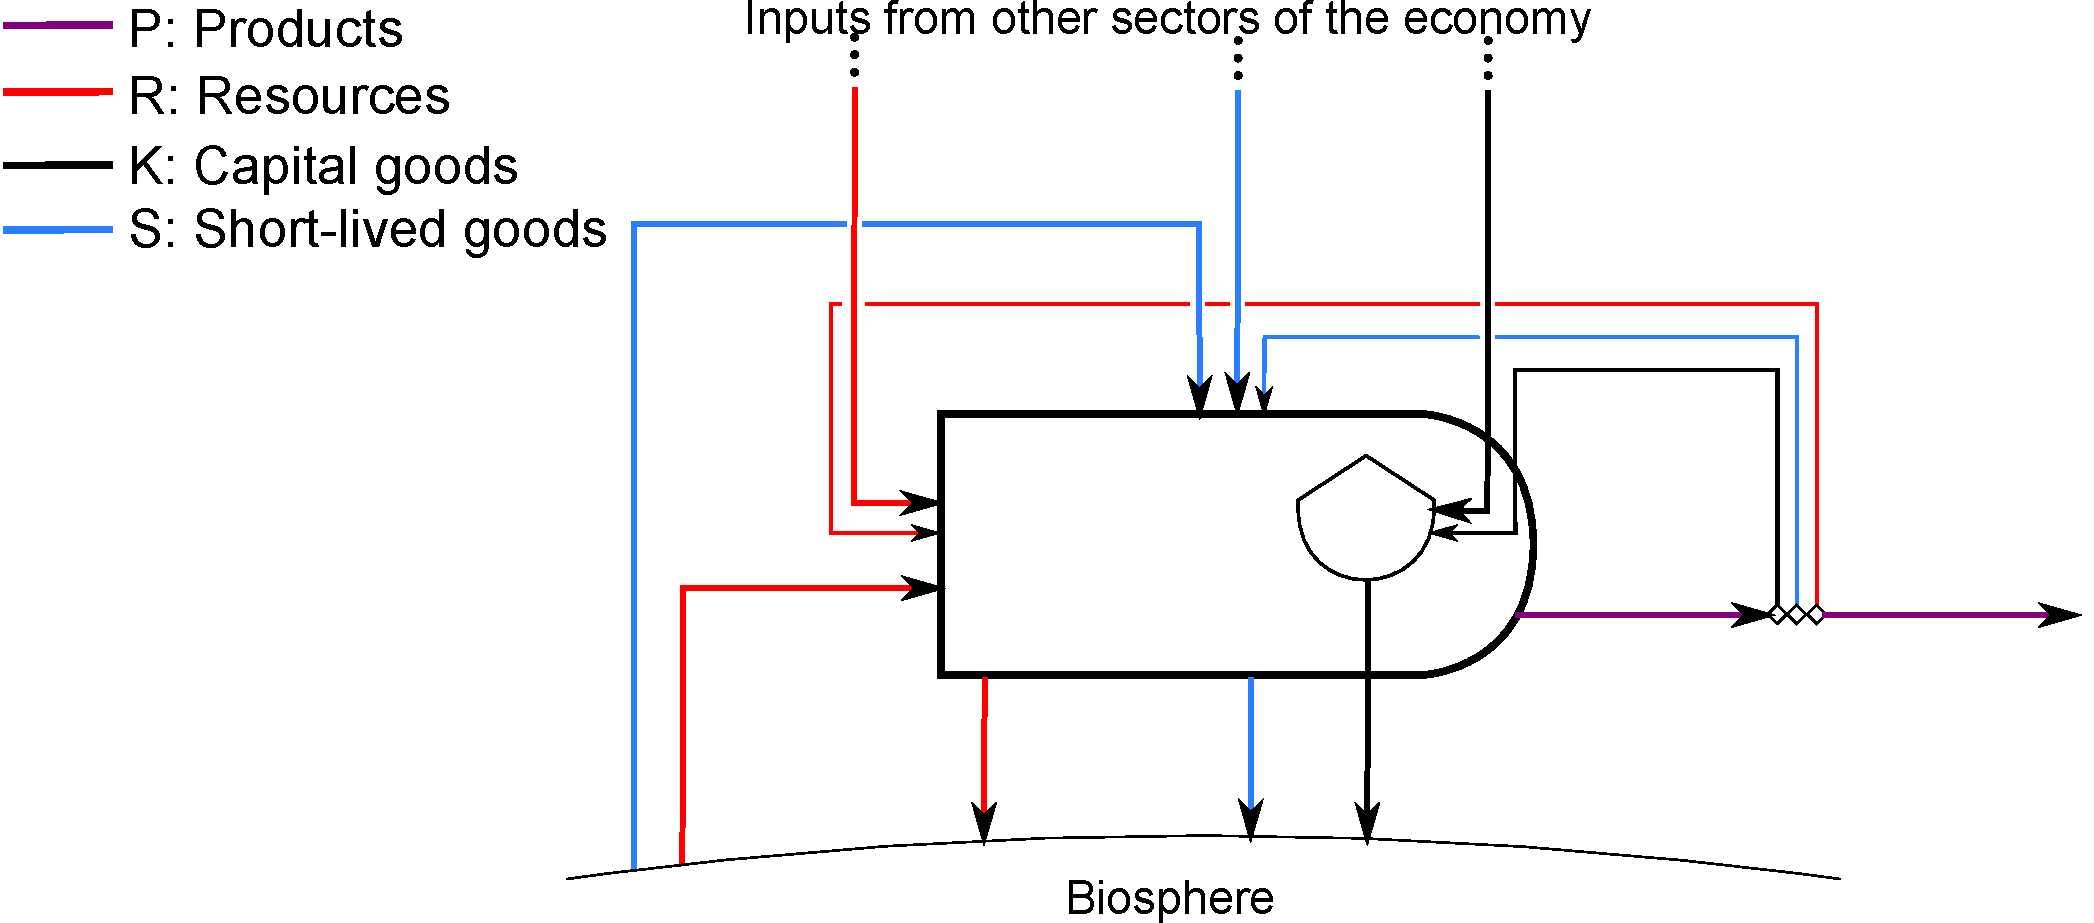
\includegraphics[width=0.8\linewidth]{Part_1/Chapter_Materials/images/PERKS_basic_unit_materials.pdf}
\caption{Material flows into and out of a single sector of the economy. Resource flows ($\dot{R}$) enter the sector from the left and are embodied in products ($\dot{P}$) which leave from the right. Some waste resources are leave the sector at the bottom and are returned to the biosphere. Short-lived material flows ($\dot{S}$) enter the sector from above and leave from below to return to the biosphere.  Only capital flows ($\dot{K}$) may accumulate within the sector, depicted by the storage tank. These also enter the sector from above. Depreciated capital leaves the sector from below and is returned to the biosphere.}
\label{fig:PERKS_materials}
\end{figure}

Resource materials ($\dot{R}$) enter the sector on the left 
and comprise those materials that are destined to be \emph{embodied} 
in the goods produced by the sector ($\dot{P}$), 
except for some proportion that are wasted.
Wastes depart from the bottom of the sector and are
returned to the biosphere. 
For example, sheet metal, rubber, and glass
(as well as many other materials) 
enter the automobile sector as resources 
and end up as material parts of the cars that are produced. 
Some fraction of these resources ($\dot{R}$) may not make it into the final product, 
such as trimming scrap from metal parts stamping, 
and may be either recycled internally, 
or wasted to the biosphere. 
Resource materials are not accumulated within a sector.

Short-lived goods ($\dot{S}$) include those materials 
that are necessary for the production processes of a sector, 
but are neither accumulated within the sector, 
nor destined to be materially part of the product of the sector. 
They enter the sector from above and leave the sector from
below and return to the biosphere. 
Examples of these short-lived flows include energy resources, such as
the electricity needed to run automobile factories,
including any contribution from labor, 
and water used by the sector. 

A number of material flows, such as production equipment,
are necessary for the continued operation of a sector 
but are not counted as short-lived goods, 
because the operation of the sector is dependent 
upon the accumulation of these materials within the sector. 
Such flows are counted as capital goods ($\dot{K}$).
Capital flows also enter from above, 
but are stored within the sector (represented by storage tanks) 
and are returned to the biosphere as capital depreciation from below.
Examples of these capital flows would be the factory and office buildings or
manufacturing equipment within the automobile industry.

All products ($\dot{P}$) leave the right of the sector. 
Some of this $\dot{P}$ flow is returned to the sector as self-consumption 
counted as resources ($\dot{R}$), 
short-lived ($\dot{S}$), or 
capital goods ($\dot{K}$); 
the remainder flows to other sectors within the economy or final demand. 
Within this view, focussing solely on material flows, energy may be accounted
as either an $\dot{R}$ flow, when the energy inflow is \emph{literally} embodied
within the outflowing product $\dot{P}$, such as crude oil converted into
gasoline within a refinery, or as an $\dot{S}$ flow, when the inflowing energy
is not literally embodied within the product. Examples include the electricity
use by an automobile factor, but also the coal or natural gas flowing into a
power plant, since the incoming chemical elements (carbon and hydrogen) \emph{do
not} travel through the electricity transmission lines.

% ****BRH says, we should say something
% about Energy here.****




%%%%%%%%%% Materials: Example A %%%%%%%%%%
\section{Example A: one sector economy}
\label{sec:A_materials}
%%%%%%%%%%

Our first example looks at the case where all processes within the economy occur within
one sector, we do not distinguish between production and consumption, as depicted in
Figure \ref{fig:A_materials}. 


\begin{figure}[h!]
\centering
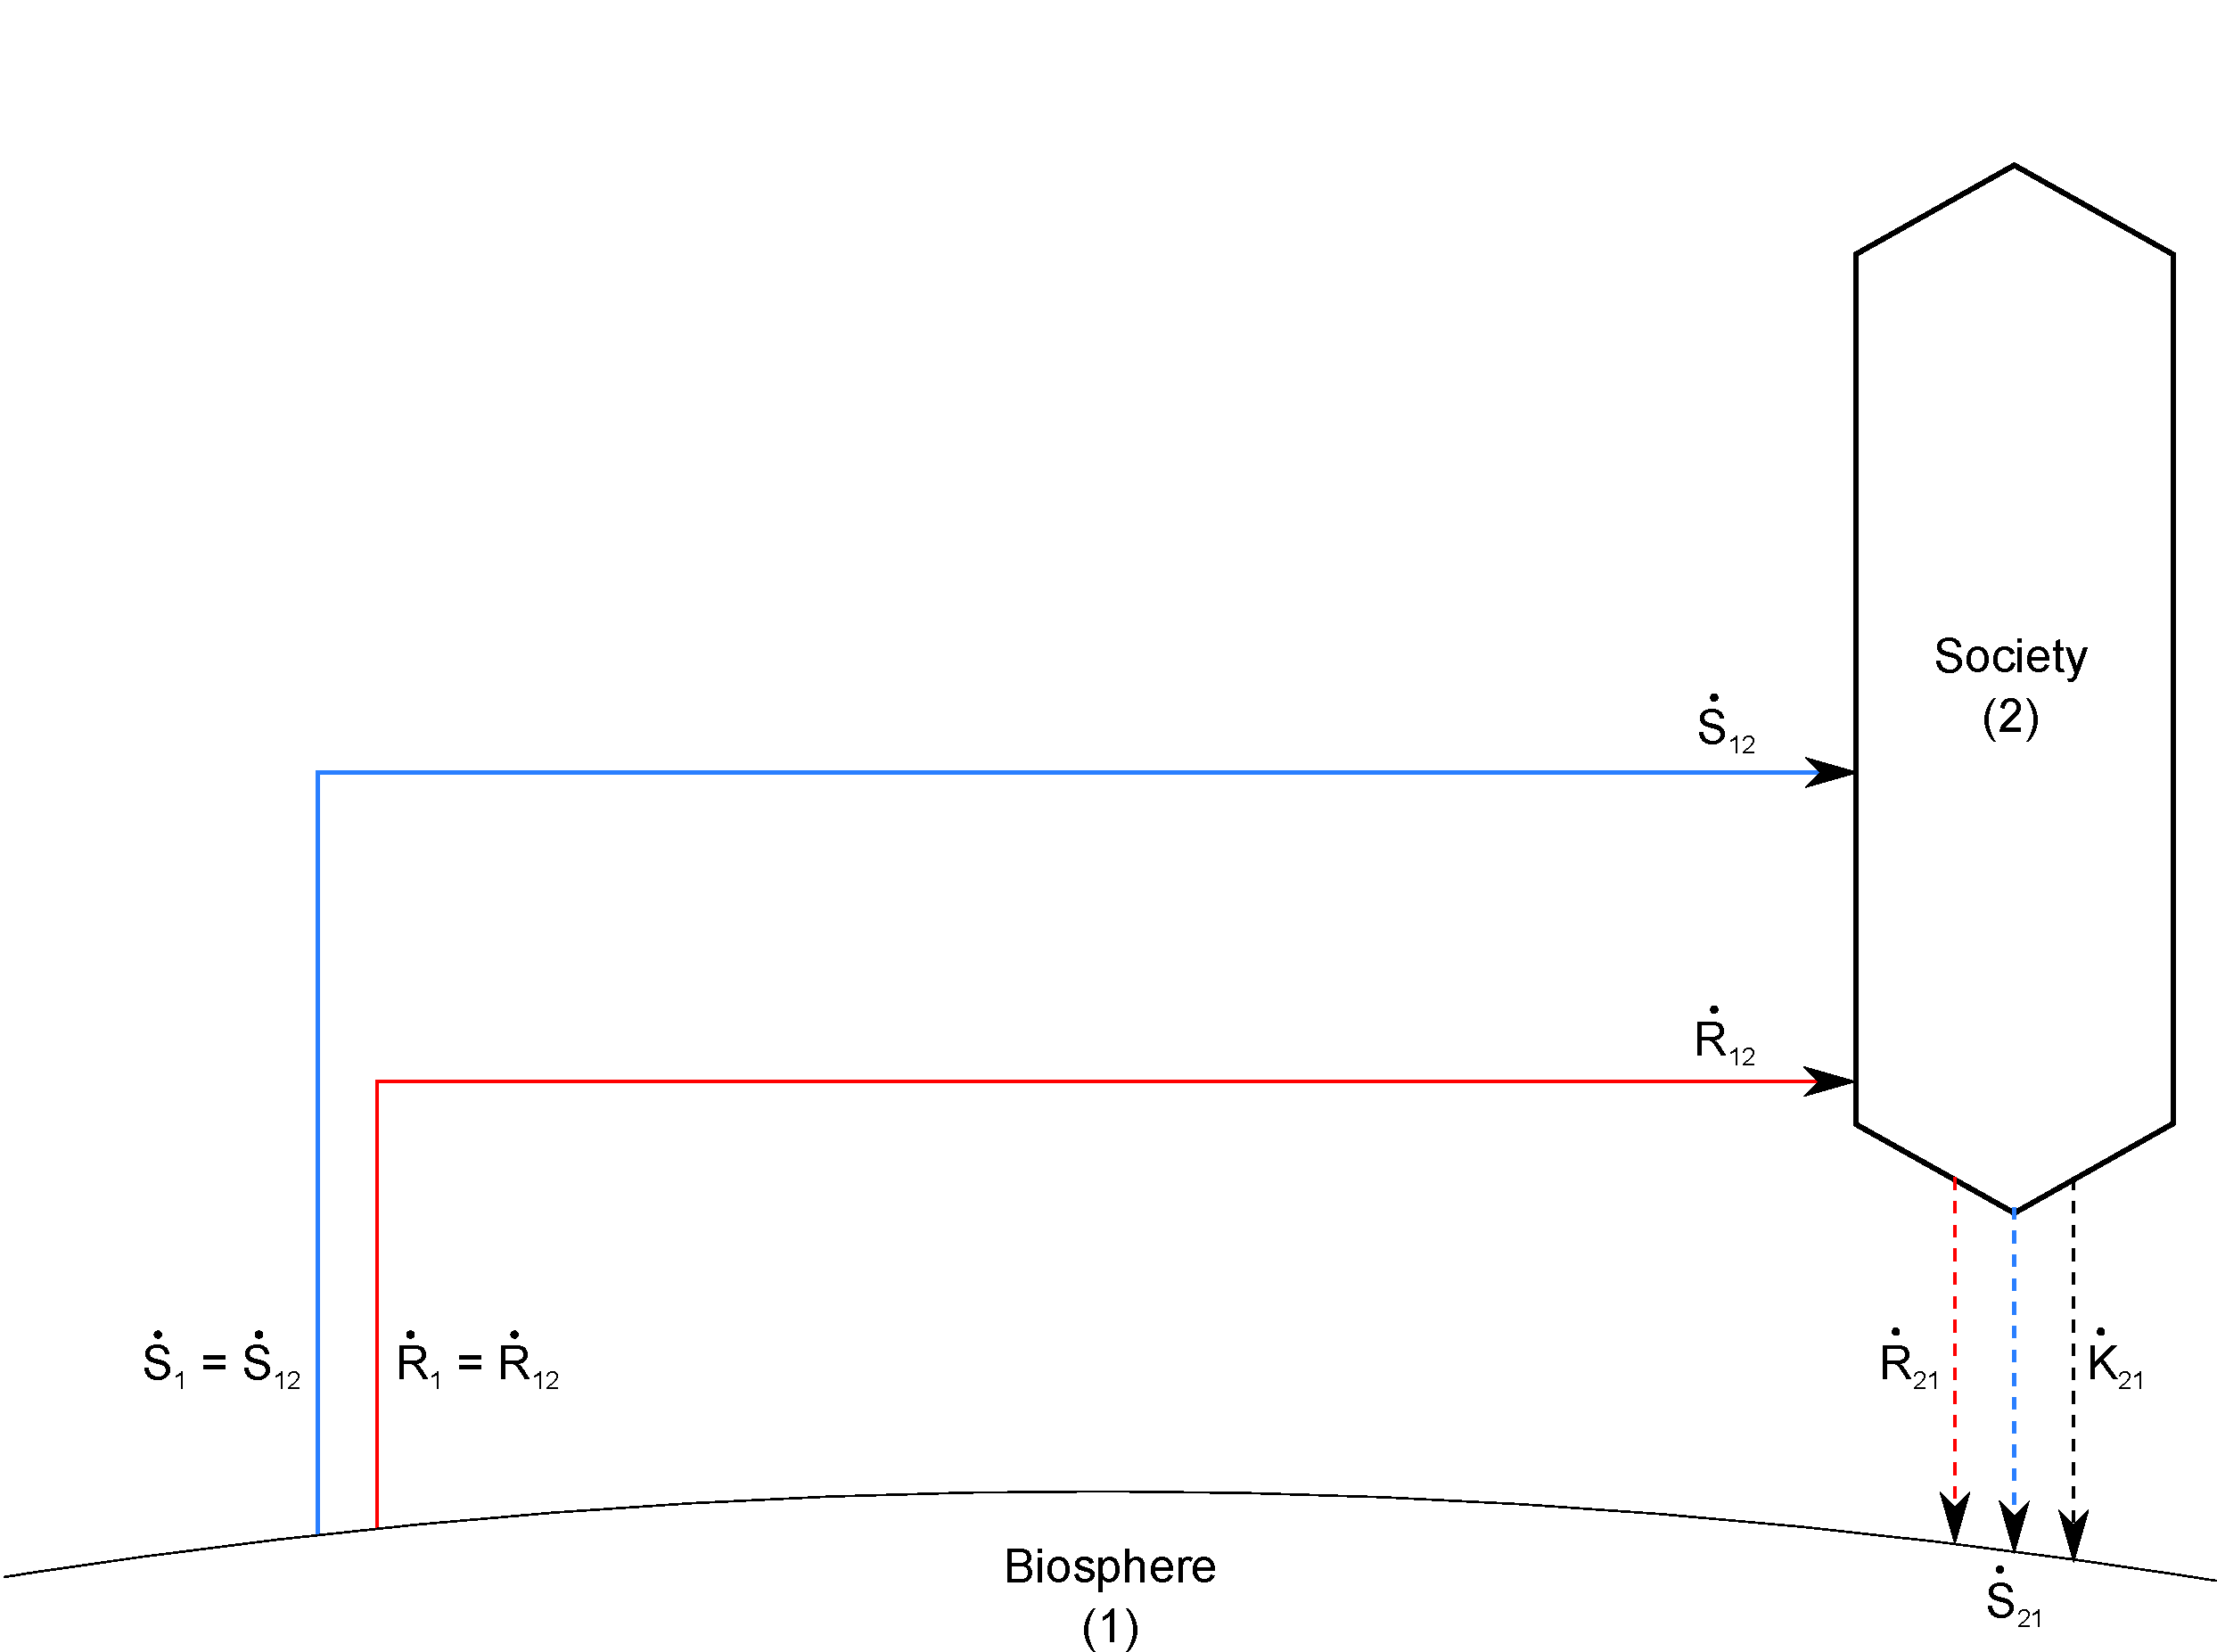
\includegraphics[width=0.8\linewidth]{Part_1/Chapter_Materials/images/1_sector_materials.pdf}
\caption{XXXX}
\label{fig:A_materials}
\end{figure}

Resources ($\dot{R}$) and short-lived materials ($\dot{S}$) flow into the economy (1) from the biosphere (0). These materials are processed within the economy into
capital goods ($\dot{K}$) which are able to be accumulated. Waste resources and used short-lived
materials are returned to the biosphere without accumulating. Capital goods are returned
to the biosphere upon depreciation.

Drawing control volumes around both the biosphere (0) and the economy (1), we can consruct
our material accounting equations, such that:

\begin{align}
\label{eq:A_CV_0_to_1}
	\frac{\mathrm{d}R_0}{\mathrm{d}t}		
	+	\frac{\mathrm{d}S_0}{\mathrm{d}t}
	+	\frac{\mathrm{d}K_0}{\mathrm{d}t}		&	
	=	\dot{R}_{10}		
	+	\dot{S}_{10}	
	+	\dot{K}_{10}											
	-	\dot{R}_{0}											
	-	\dot{S}_{0}								\\
\label{eq:A_CV_0_to_1a}
	\frac{\mathrm{d}R_{1}}{\mathrm{d}t}
	+ \frac{\mathrm{d}S_{1}}{\mathrm{d}t}
	+ \frac{\mathrm{d}K_{1}}{\mathrm{d}t}		&
	= \dot{R}_{01} 
	+ \dot{S}_{01} + \dot{S}_{11}
	- \dot{S}_{1}				
	- \dot{R}_{10}				
	- \dot{S}_{10}				
	- \dot{K}_{10}											
\end{align}

\noindent Remembering that neither resources nor short-lived goods accumulate within economic sectors, tells us that:

\begin{equation}\label{eq:A-dS_1/dt_zero}
	\frac{\mathrm{d}S_1}{\mathrm{d}t}
	= \frac{\mathrm{d}R_1}{\mathrm{d}t}
	= 0.
\end{equation}

\noindent Additionally, we may also say that:

\begin{equation}\label{eq:A_S11}
	\dot{S}_{11} = \dot{S}_{1},
\end{equation}

\noindent such that our material accumulation ****BRH says, shouldn't this word be
"accounting" -- not accumulation -- given that is what we
called it in the sentence introducing eq. 2.4. Or, should we change "accounting" above to accumulation?
Or, are they synonyms? And, aren't there two of these equations? 2.4 and 2.5? I added a separate
label for eqn. 2.5**** equations \ref{eq:A_CV_0_to_1} and \ref{eq:A_CV_0_to_1a} 
become:

\begin{align}\label{eq:A_CV_0_to_1_b}
	\frac{\mathrm{d}R_0}{\mathrm{d}t}		
	+	\frac{\mathrm{d}S_0}{\mathrm{d}t}
	+	\frac{\mathrm{d}K_0}{\mathrm{d}t}		&	
	=	\dot{R}_{10}		
	+	\dot{S}_{10}	
	+	\dot{K}_{10}											
	-	\dot{R}_{0}											
	-	\dot{S}_{0}								\\
	\frac{\mathrm{d}K_{1}}{\mathrm{d}t}		&
	= \dot{R}_{01} 
	+ \dot{S}_{01} 
	- \dot{R}_{10}				
	- \dot{S}_{10}				
	- \dot{K}_{10}											
\end{align}

\noindent Because the only "capital" that accumulates in the biosphere is that which is a waste flow (capital depreciation)
from the economy, e.g. worn-out machines in the scrap yard, we may say that:

\begin{equation} \label{eq:A_K0_balance}
	\frac{\mathrm{d}K_{0}}{\mathrm{d}t}		
	= \dot{K}_{10}
\end{equation}


%%%%%%%%%% Materials: Example B %%%%%%%%%%
\newpage
\section{Example B: two sector economy}
\label{sec:B_materials}
%%%%%%%%%%

In our second example B, we split society into two sectors: production and consumption as depicted in Figure \ref{fig:B_materials}. 

\begin{figure}[h!]
\centering
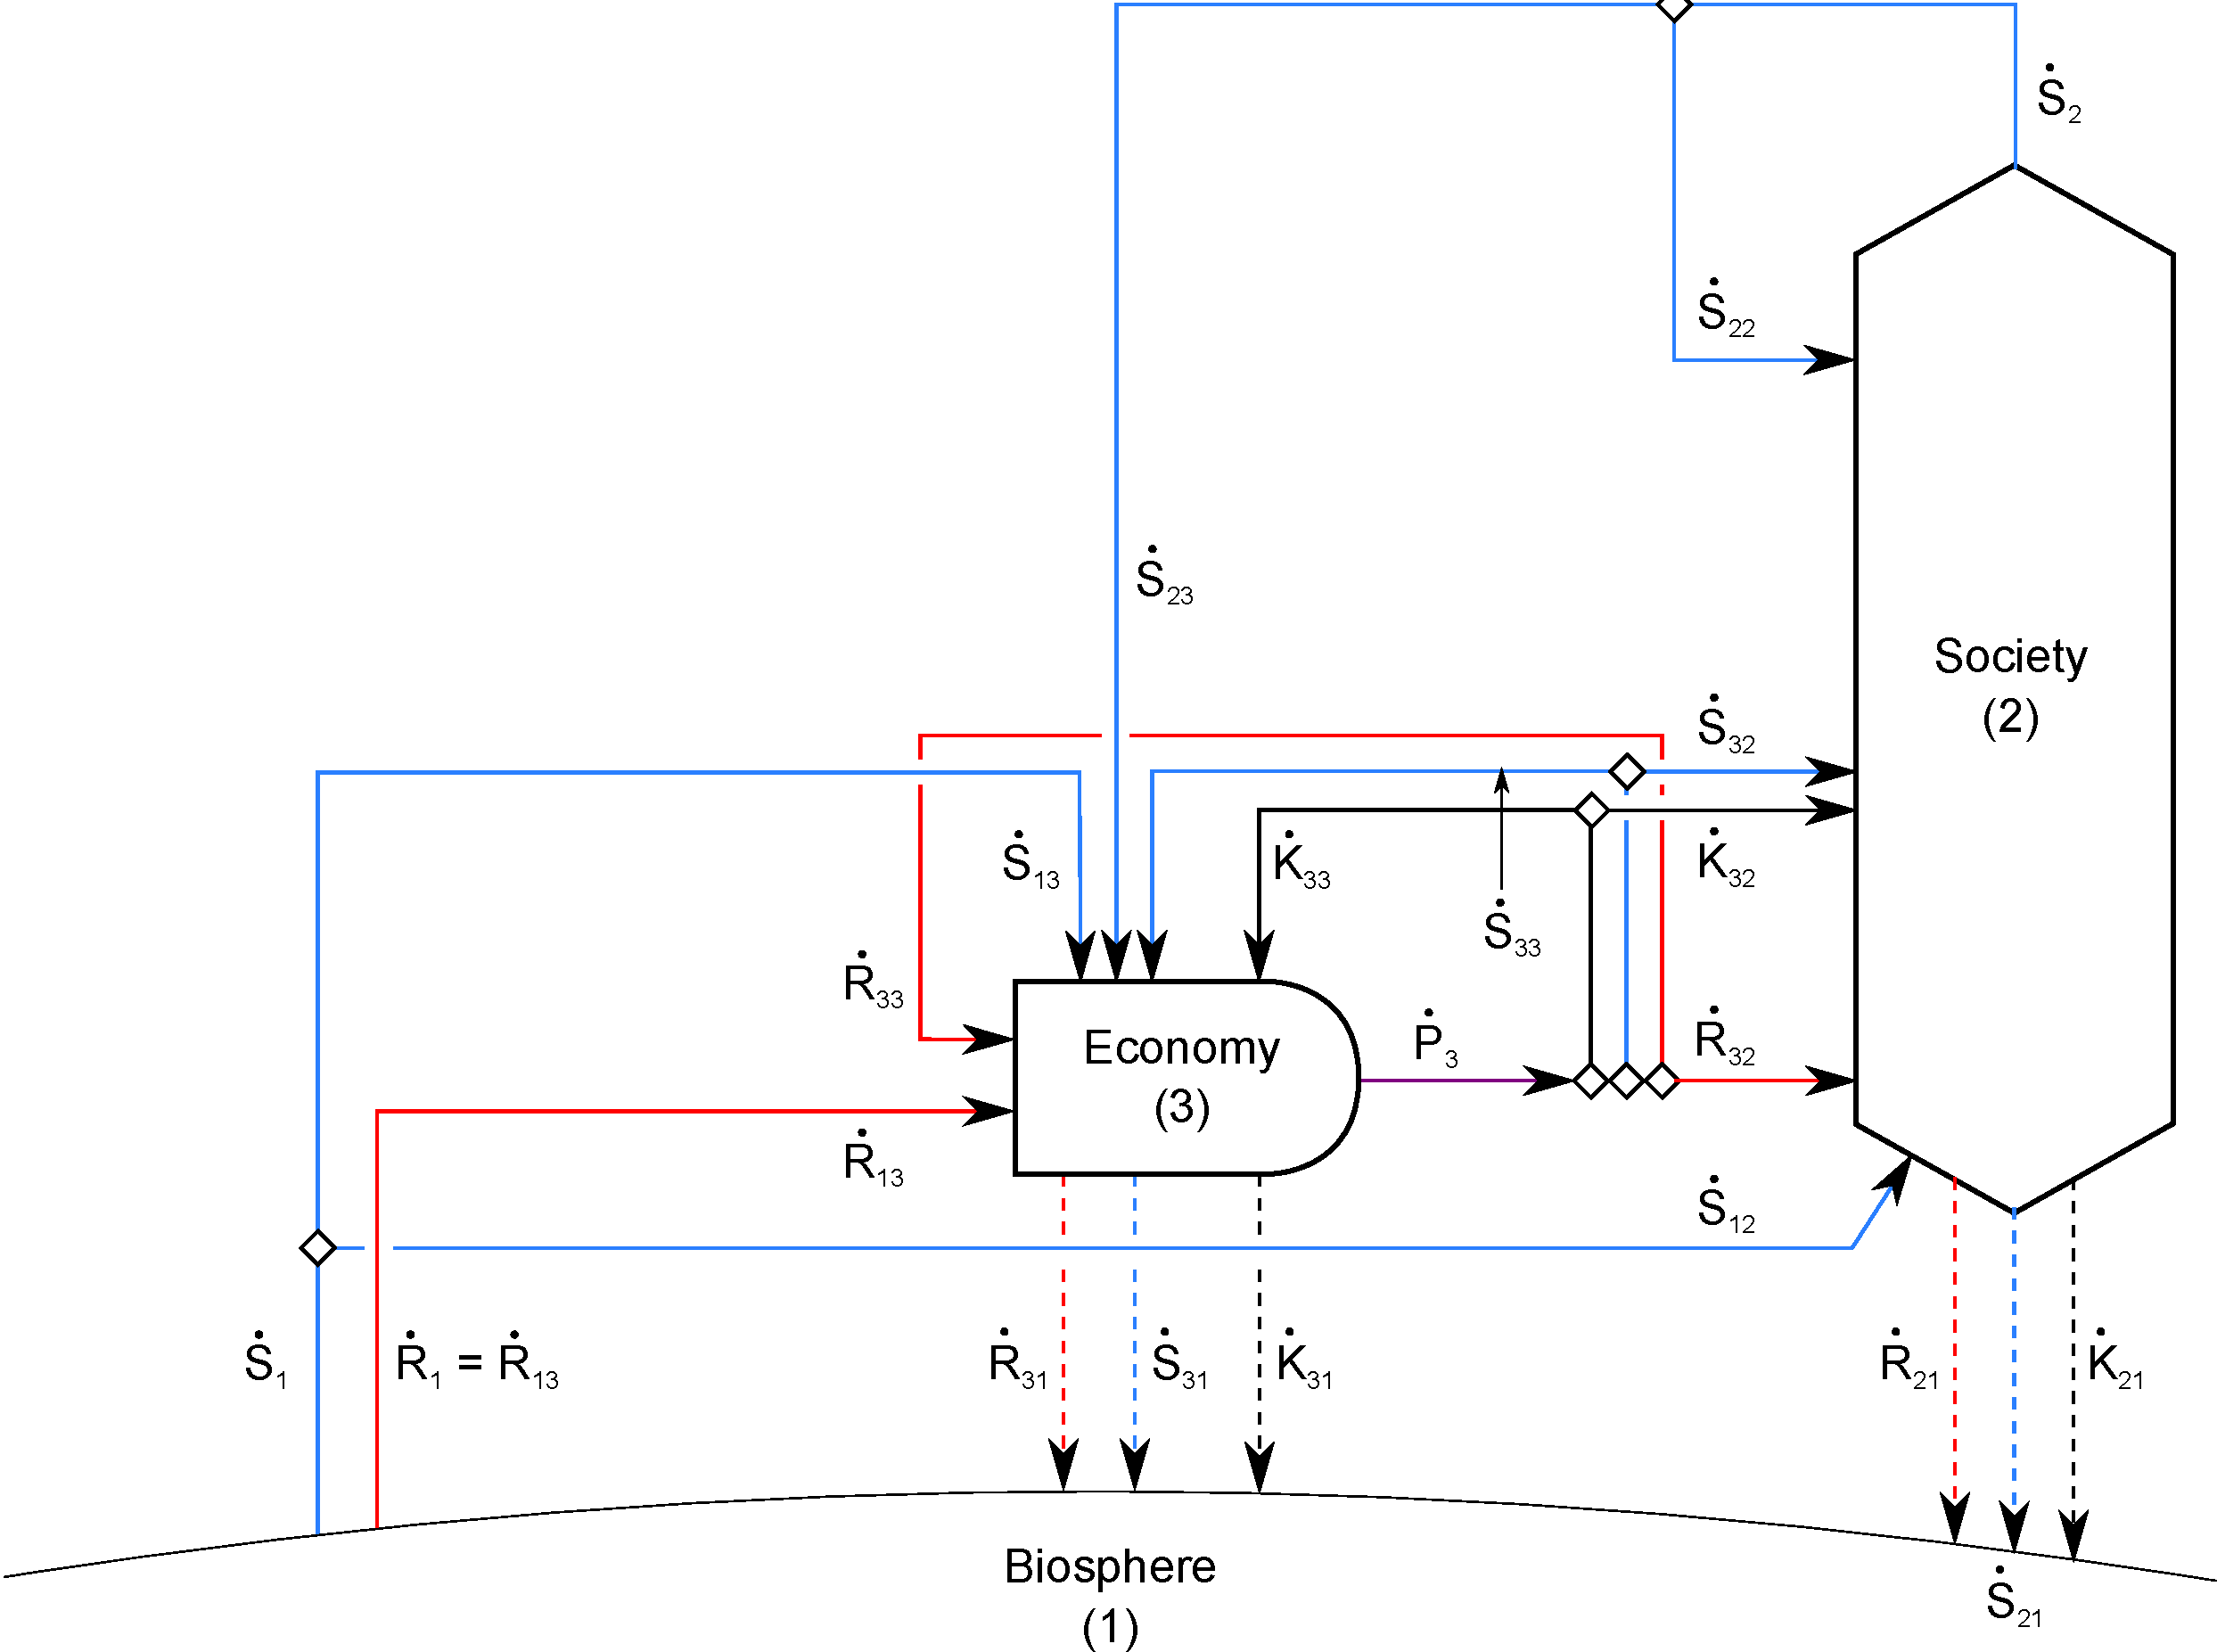
\includegraphics[width=0.8\linewidth]{Part_1/Chapter_Materials/images/2_sector_materials.pdf}
\caption{XXXX}
\label{fig:B_materials}
\end{figure}

Sector 2 produces goods and services for consumption in society (1). Again, setting control volumes around the biosphere and our two sectors, our accumulation equations are now written:

\begin{align} \label{eq:B_CV_0_to_2}
	\frac{\mathrm{d}R_{0}}{\mathrm{d}t} 
	+ \frac{\mathrm{d}S_{0}}{\mathrm{d}t}	
	+ \frac{\mathrm{d}K_0}{\mathrm{d}t}		&
	=  \dot{R}_{10} + \dot{R}_{20} 
	+ \dot{S}_{10} + \dot{S}_{20} 
	+ \dot{K}_{10} + \dot{K}_{20} 
	- \dot{R}_{0} 
	- \dot{S}_{0} 							\\
	\frac{\mathrm{d}R_{1}}{\mathrm{d}t} 
	+ \frac{\mathrm{d}S_{1}}{\mathrm{d}t}	
	+ \frac{\mathrm{d}K_{1}}{\mathrm{d}t}	&
	=  \dot{R}_{21} 
	+ \dot{S}_{01} 
	+ \dot{S}_{11} 
	+ \dot{S}_{21}
	+ \dot{K}_{21}
	- \dot{S}_{1} 
	- \dot{R}_{10} 
	- \dot{S}_{10} 
	- \dot{K}_{10},							\\
	\frac{\mathrm{d}R_{2}}{\mathrm{d}t} 
	+ \frac{\mathrm{d}S_{2}}{\mathrm{d}t}
	+ \frac{\mathrm{d}K_{2}}{\mathrm{d}t}	&
	=  \dot{R}_{02} 
	+ \dot{R}_{22} 
	+ \dot{S}_{02} 
	+ \dot{S}_{12} 
	+ \dot{S}_{22} 
	+ \dot{K}_{22}
	- \dot{P}_{2}
	- \dot{R}_{20} 
	- \dot{S}_{20} 
	- \dot{K}_{20},
\end{align}

\begin{equation}
	\dot{R}_{0} = \dot{R}_{02}
\end{equation}

\begin{align}\label{eq:B_S_def}
	\dot{S}_{0} = 
	& \dot{S}_{01} + \dot{S}_{02};
	& \dot{S}_{1} = 
	\dot{S}_{11} + \dot{S}_{12}
\end{align}

Since only capital flows ($\dot{K}$) may be accumulated and are dependent only on flows of capital in and depreciation of capital, we may define capital balance equations:

\begin{equation} \label{eq:B_K1_balance}
	\frac{\mathrm{d}K_{1}}{\mathrm{d}t}
	=  \dot{K}_{12} - \dot{K}_{20},
\end{equation}

[NOT SURE IF THIS IS TRUE IF WE THINK OF $\dot{R}_{12}$ AS FOOD AND $K_{1}$ AS INCLUDING HUMANS... YES, I THINK $\dot{R}_{12}$ CAN BE TURNED INTO  $\dot{K}_{1}$ INTERNALLY, AS THE ACCUMULATION OF (LITERAL) HUMAN CAPITAL, I.E. POPULATION]

\begin{equation} \label{eq:B_K2_balance}
	\frac{\mathrm{d}K_{2}}{\mathrm{d}t}
	=  \dot{K}_{22} - \dot{K}_{20},
\end{equation}

\begin{equation} \label{eq:B_P_def}
	\dot{P}_{2}
	= \dot{R}_{21}
	+ \dot{R}_{22}
	+ \dot{S}_{21}
	+ \dot{S}_{22}
	+ \dot{K}_{21}	 
	+ \dot{K}_{22},
\end{equation}


\noindent Again, remembering that resources and short-lived
goods do not accumulate within sectors of the economy:

\begin{equation}\label{eq:dR_and_dS_zero}
	\frac{\mathrm{d}R_{1}}{\mathrm{d}t}
	= \frac{\mathrm{d}R_{2}}{\mathrm{d}t} 
	= \frac{\mathrm{d}S_{1}}{\mathrm{d}t} 
	= \frac{\mathrm{d}S_{2}}{\mathrm{d}t} 
	= 0,
\end{equation}

\noindent and substituting equations \ref{eq:B_S_def},
\ref{eq:B_K2_balance}  and \ref{eq:B_P_def}, our balance 
equations may now be written:


\begin{align} \label{eq:B_CV_0_to_2_b}
	\frac{\mathrm{d}R_{0}}{\mathrm{d}t} 
	+ \frac{\mathrm{d}S_{0}}{\mathrm{d}t}	
	+ \frac{\mathrm{d}K_0}{\mathrm{d}t}		
	& = \dot{R}_{10} + \dot{R}_{20} 
	+ \dot{S}_{10} + \dot{S}_{20} 
	+ \dot{K}_{10} + \dot{K}_{20} 
	- \dot{R}_{0} 
	- \dot{S}_{0} 							\\
	\frac{\mathrm{d}K_{1}}{\mathrm{d}t}	
	& = \dot{R}_{21} 
	+ \dot{S}_{01} 
	+ \dot{S}_{21}
	+ \dot{K}_{21}
	- \dot{S}_{12} 
	- \dot{R}_{10} 
	- \dot{S}_{10} 
	- \dot{K}_{10},							\\
	\dot{K}_{22} - \dot{K}_{20}	
	& = \dot{R}_{02} 
	+ \dot{S}_{02} 
	+ \dot{S}_{12} 
	- \dot{R}_{21}
	- \dot{S}_{21}
	- \dot{K}_{21}
	- \dot{R}_{20} 
	- \dot{S}_{20} 
	- \dot{K}_{20}							\\
\end{align}





%%%%%%%%%% Materials: Example C %%%%%%%%%%
\newpage
\section{Example C: three sector economy}
\label{sec:C_materials}
%%%%%%%%%%

In example C, we differentiate between two production sectors, one produces energy and one produces other goods and services.

\begin{figure}[h!]
\centering
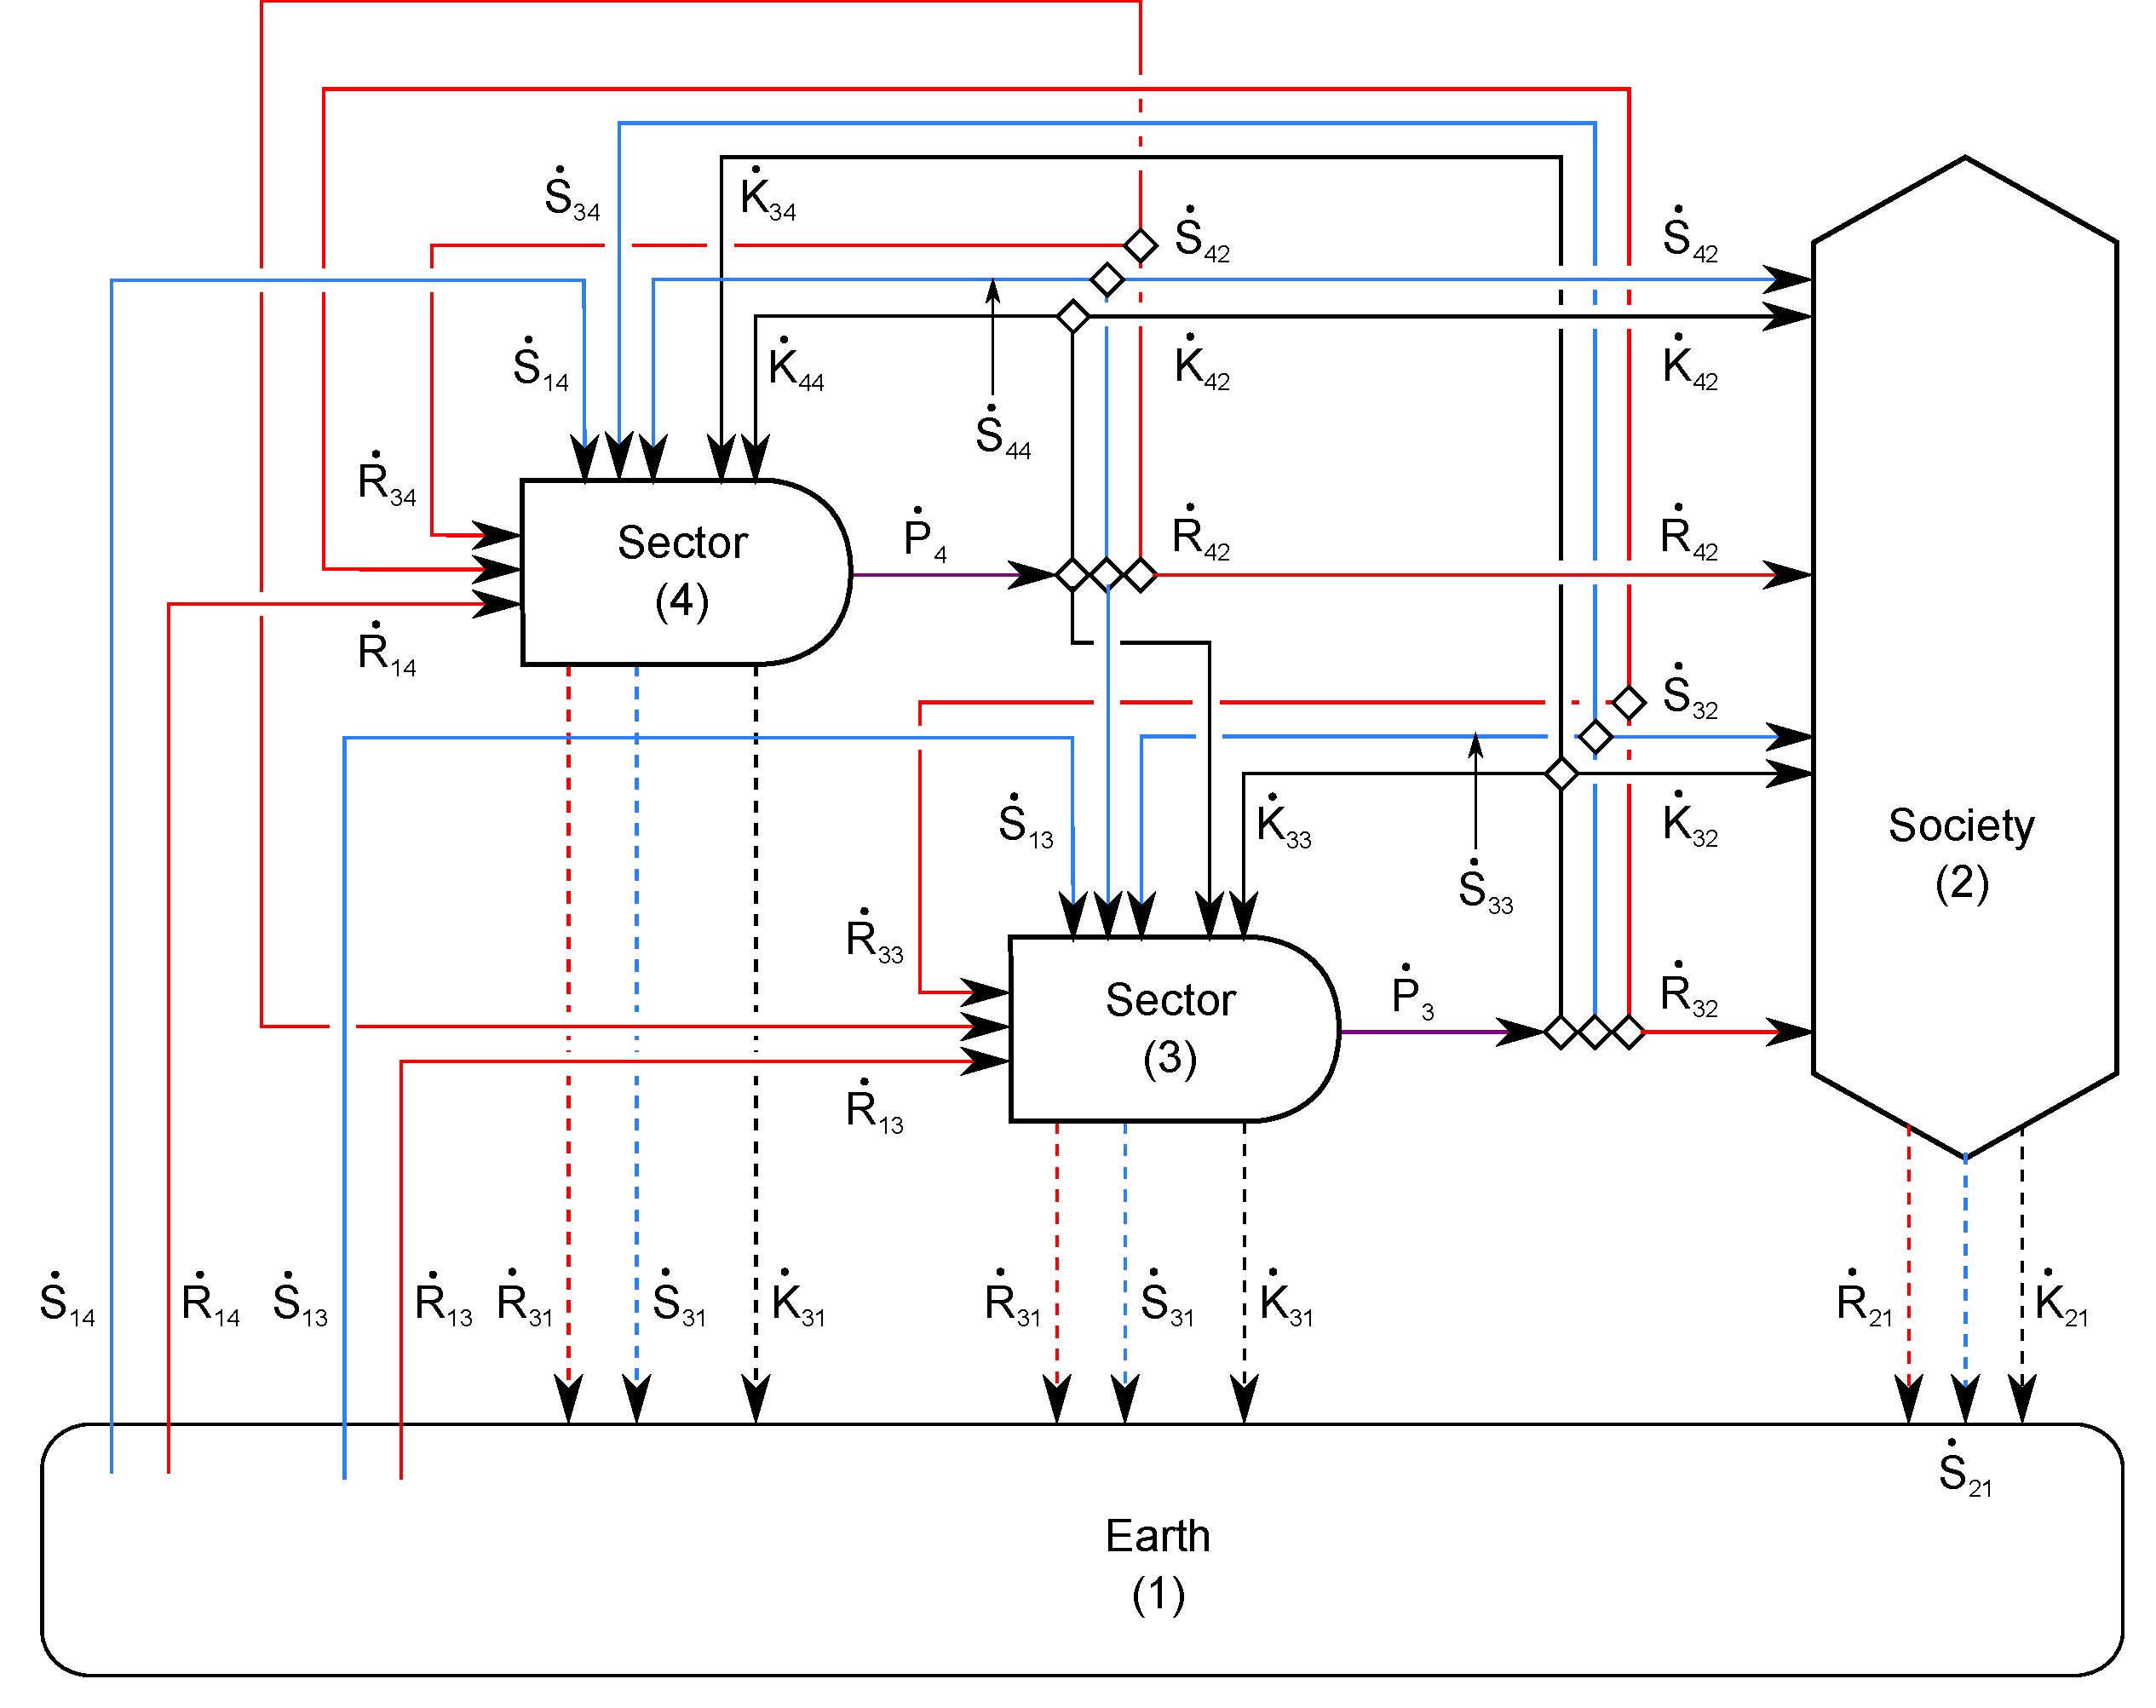
\includegraphics[width=0.8\linewidth]{Part_1/Chapter_Materials/images/3_sector_materials.pdf}
\caption{XXXX}
\label{fig:C_materials}
\end{figure}

\begin{equation} \label{eq:C-CV_R_dot_0a}
	\frac{\mathrm{d}R_{0}}{\mathrm{d}t} 
	+ \frac{\mathrm{d}S_{0}}{\mathrm{d}t}	
	+ \frac{\mathrm{d}K_0}{\mathrm{d}t}
	=  \dot{R}_{10} + \dot{R}_{20} + \dot{R}_{30}
	+ \dot{S}_{10} + \dot{S}_{20} + \dot{S}_{30}
	+ \dot{K}_{10} + \dot{K}_{20} + \dot{K}_{30}
	- \dot{R}_{0} 
	- \dot{S}_{0},
\end{equation}

\begin{equation}
	\dot{R}_{0} = \dot{R}_{02} + \dot{R}_{03}
\end{equation}

\begin{equation}
	\dot{S}_{0} = \dot{S}_{01} + \dot{S}_{02} + \dot{S}_{03}
\end{equation}

 \begin{equation} \label{eq:C-CV_R_dot_0b}
 	\frac{\mathrm{d}R_{0}}{\mathrm{d}t} 
 	+ \frac{\mathrm{d}S_{0}}{\mathrm{d}t}	
 	+ \frac{\mathrm{d}K_0}{\mathrm{d}t}
 	=  \dot{R}_{10} + \dot{R}_{20} + \dot{R}_{30}
 	+ \dot{S}_{10} + \dot{S}_{20} + \dot{S}_{30}
 	+ \dot{K}_{10} + \dot{K}_{20} + \dot{K}_{30}
 	- \dot{R}_{02} - \dot{R}_{03} 
 	- \dot{S}_{01} - \dot{S}_{02} - \dot{S}_{03},
 \end{equation}
 
 \begin{equation} \label{eq:C-CV_R_dot_1}
 	\frac{\mathrm{d}R_{1}}{\mathrm{d}t} 
	+ \frac{\mathrm{d}S_{1}}{\mathrm{d}t}
 	+ \frac{\mathrm{d}K_{1}}{\mathrm{d}t}
 	=  \dot{R}_{21} + \dot{R}_{31}
 	+ \dot{S}_{01} + \dot{S}_{11} 
	+ \dot{S}_{21} + \dot{S}_{31}
 	+ \dot{K}_{21} + \dot{K}_{31}
 	- \dot{S}_{1} 
	- \dot{R}_{10} 
 	- \dot{S}_{10} 
 	- \dot{K}_{10},
 \end{equation}
 
 \begin{equation} \label{eq:C-CV_R_dot_2}
 	\frac{\mathrm{d}R_{2}}{\mathrm{d}t} 
	+ \frac{\mathrm{d}S_{2}}{\mathrm{d}t}
 	+ \frac{\mathrm{d}K_{2}}{\mathrm{d}t}
 	=  \dot{R}_{02} + \dot{R}_{22} + \dot{R}_{32}
 	+ \dot{S}_{02} + \dot{S}_{12} 
	+ \dot{S}_{22} + \dot{S}_{32} 
 	+ \dot{K}_{22} + \dot{K}_{32}
 	- \dot{P}_{2}
 	- \dot{R}_{20} 
 	- \dot{S}_{20} 
 	- \dot{K}_{20},
 \end{equation}
 
 \begin{equation} \label{eq:C-CV_R_dot_3}
 	\frac{\mathrm{d}R_{3}}{\mathrm{d}t} 
	+ \frac{\mathrm{d}S_{3}}{\mathrm{d}t}
 	+ \frac{\mathrm{d}K_{3}}{\mathrm{d}t}
 	=  \dot{R}_{03} + \dot{R}_{23} + \dot{R}_{33}
 	+ \dot{S}_{03} + \dot{S}_{13} 
	+ \dot{S}_{23} + \dot{S}_{33} 
 	+ \dot{K}_{23} + \dot{K}_{33}
 	- \dot{P}_{3}
 	- \dot{R}_{30} 
 	- \dot{S}_{30} 
 	- \dot{K}_{30},
 \end{equation}

\begin{equation}\label{eq:C-dR_dt_zero}
	\frac{\mathrm{d}R_{1}}{\mathrm{d}t} = \frac{\mathrm{d}R_{2}}{\mathrm{d}t} = \frac{\mathrm{d}R_{3}}{\mathrm{d}t} = 0
\end{equation}

\begin{equation}\label{eq:C-dS_dt_zero}
	\frac{\mathrm{d}S_{1}}{\mathrm{d}t} = \frac{\mathrm{d}S_{2}}{\mathrm{d}t} = \frac{\mathrm{d}S_{3}}{\mathrm{d}t} = 0
\end{equation}

\begin{equation} \label{eq:C-CV_K_dot_2}
	\frac{\mathrm{d}K_{2}}{\mathrm{d}t}
	=  \dot{K}_{22} + \dot{K}_{32} 
	- \dot{K}_{20},
\end{equation}

\begin{equation} \label{eq:C-CV_K_dot_3}
	\frac{\mathrm{d}K_{2}}{\mathrm{d}t}
	=  \dot{K}_{23} + \dot{K}_{33} 
	- \dot{K}_{30},
\end{equation}

 \begin{equation} \label{eq:C-CV_R_dot_1b}
 	\frac{\mathrm{d}K_{1}}{\mathrm{d}t}
 	=  \dot{R}_{21} + \dot{R}_{31}
 	+ \dot{S}_{01} + \dot{S}_{11} 
	+ \dot{S}_{21} + \dot{S}_{31}
 	+ \dot{K}_{21} + \dot{K}_{31}
 	- \dot{S}_{1} 
	- \dot{R}_{10} 
 	- \dot{S}_{10} 
 	- \dot{K}_{10},
 \end{equation}
 
 \begin{equation} \label{eq:C-CV_R_dot_2b}
 	\frac{\mathrm{d}K_{2}}{\mathrm{d}t}
 	=  \dot{R}_{02} + \dot{R}_{22} + \dot{R}_{32}
 	+ \dot{S}_{02} + \dot{S}_{12} 
	+ \dot{S}_{22} + \dot{S}_{32} 
 	+ \dot{K}_{22} + \dot{K}_{32}
 	- \dot{P}_{2}
 	- \dot{R}_{20} 
 	- \dot{S}_{20} 
 	- \dot{K}_{20}
	=  \dot{K}_{22} + \dot{K}_{32} 
	- \dot{K}_{20},
 \end{equation}
 
 \begin{equation} \label{eq:C-CV_R_dot_3}
 	\frac{\mathrm{d}K_{3}}{\mathrm{d}t}
 	=  \dot{R}_{03} + \dot{R}_{23} + \dot{R}_{33}
 	+ \dot{S}_{03} + \dot{S}_{13} 
	+ \dot{S}_{23} + \dot{S}_{33} 
 	+ \dot{K}_{23} + \dot{K}_{33}
 	- \dot{P}_{3}
 	- \dot{R}_{30} 
 	- \dot{S}_{30} 
 	- \dot{K}_{30}
	=  \dot{K}_{23} + \dot{K}_{33} 
	- \dot{K}_{30},
 \end{equation}




\begin{figure}[h!]
\centering
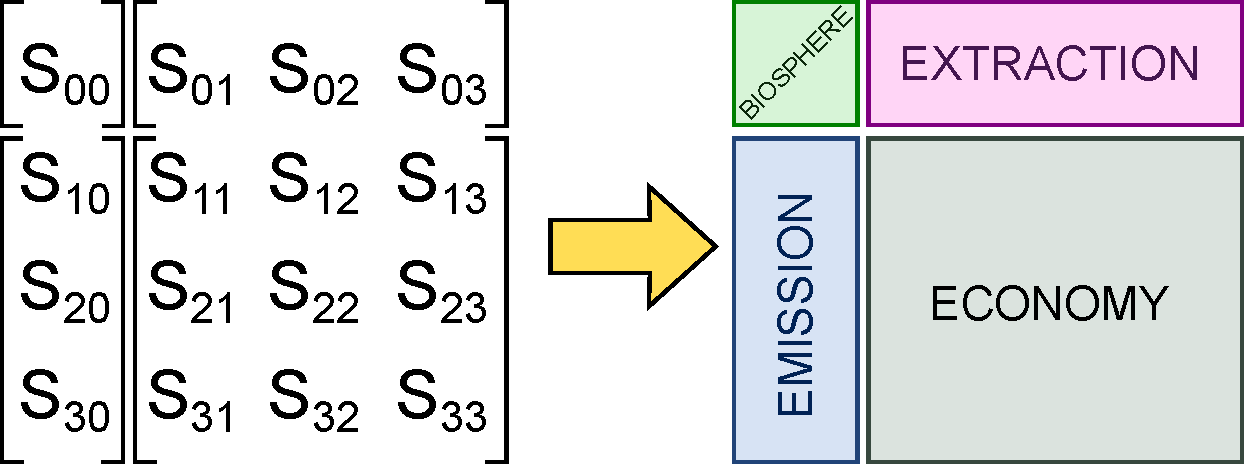
\includegraphics[width=0.8\linewidth]{Part_1/Chapter_Materials/images/Matrix.pdf}
\caption{XXXX}
\label{fig:C_mat_matrix}
\end{figure}

%%%%%%%%%% Materials: Auto industry example %%%%%%%%%%
\section{Materials in the auto industry}
\label{sec:materials_auto}
%%%%%%%%%%

%%%%%%%%%% Materials: Summary %%%%%%%%%%
\section{Summary}
\label{sec:materials_summary}
%%%%%%%%%%

\bibliography{../../EROI_review_v2}
\bibliographystyle{unsrt}


% Always give a unique label
% and use \ref{<label>} for cross-references
% and \cite{<label>} for bibliographic references
% use \sectionmark{}
% to alter or adjust the section heading in the running head
%% Instead of simply listing headings of different levels we recommend to let every heading be followed by at least a short passage of text. Furtheron please use the \LaTeX\ automatism for all your cross-references and citations.

%% Please note that the first line of text that follows a heading is not indented, whereas the first lines of all sequent paragraphs are.

%% Use the standard \verb|equation| environment to typeset your equations, e.g.
%
%% \begin{equation}
%% a \times b = c\;,
%% \end{equation}
%
%% however, for multiline equations we recommend to use the \verb|eqnarray|
%% environment\footnote{In physics texts please activate the class option \texttt{vecphys} to depict your vectors in \textbf{\itshape boldface-italic} type - as is customary for a wide range of physical jects.}.
%%\begin{eqnarray}
%%a \times b = c \nonumber\\
%% \vec{a} \cdot \vec{b}=\vec{c}
%% \label{eq:01}
%%\end{eqnarray}

%% \section{section Heading}
%% \label{sec:2}
%% Instead of simply listing headings of different levels we recommend to let every heading be followed by at least a short passage of text. Furtheron please use the \LaTeX\ automatism for all your cross-references\index{cross-references} and citations\index{citations} as has already been described in Sect.~\ref{sec:2}.

%% \begin{quotation}
%% Please do not use quotation marks when quoting texts! Simply use the \verb|quotation| environment -- it will automatically render Springer's preferred layout.
%% \end{quotation}


%% \section{section Heading}
%% Instead of simply listing headings of different levels we recommend to let every heading be followed by at least a short passage of text. Furtheron please use the \LaTeX\ automatism for all your cross-references and citations as has already been described in Sect.~\ref{sec:2}, see also Fig.~\ref{fig:1}\footnote{If you copy text passages, figures, or tables from other works, you must obtain \textit{permission} from the copyright holder (usually the original publisher). Please enclose the signed permission with the manucript. The sources\index{permission to print} must be acknowledged either in the captions, as footnotes or in a separate section of the book.}

%% Please note that the first line of text that follows a heading is not indented, whereas the first lines of all sequent paragraphs are.

% For figures use
%
%% \begin{figure}[b]
%% \sidecaption
% Use the relevant command for your figure-insertion program
% to insert the figure file.
% For example, with the option graphics use
%% \includegraphics[scale=.65]{figure}
%
% If not, use
%\picplace{5cm}{2cm} % Give the correct figure height and width in cm
%
%% \caption{If the width of the figure is less than 7.8 cm use the \texttt{sidecapion} command to flush the caption on the left side of the page. If the figure is positioned at the top of the page, align the sidecaption with the top of the figure -- to achieve this you simply need to use the optional argument \texttt{[t]} with the \texttt{sidecaption} command}
%% \label{fig:1}       % Give a unique label
%% \end{figure}


%% \paragraph{Paragraph Heading} %
%% Instead of simply listing headings of different levels we recommend to let every heading be followed by at least a short passage of text. Furtheron please use the \LaTeX\ automatism for all your cross-references and citations as has already been described in Sect.~\ref{sec:2}.

%% Please note that the first line of text that follows a heading is not indented, whereas the first lines of all sequent paragraphs are.

%% For typesetting numbered lists we recommend to use the \verb|enumerate| environment -- it will automatically render Springer's preferred layout.

%% \begin{enumerate}
%% \item{Livelihood and survival mobility are oftentimes coutcomes of uneven socioeconomic development.}
%% \begin{enumerate}
%% \item{Livelihood and survival mobility are oftentimes coutcomes of uneven socioeconomic development.}
%% \item{Livelihood and survival mobility are oftentimes coutcomes of uneven socioeconomic development.}
%% \end{enumerate}
%% \item{Livelihood and survival mobility are oftentimes coutcomes of uneven socioeconomic development.}
%% \end{enumerate}


%% \paragraph{paragraph Heading} In order to avoid simply listing headings of different levels we recommend to let every heading be followed by at least a short passage of text. Use the \LaTeX\ automatism for all your cross-references and citations as has already been described in Sect.~\ref{sec:2}, see also Fig.~\ref{fig:2}.

%% Please note that the first line of text that follows a heading is not indented, whereas the first lines of all sequent paragraphs are.

%% For unnumbered list we recommend to use the \verb|itemize| environment -- it will automatically render Springer's preferred layout.

%% \begin{itemize}
%% \item{Livelihood and survival mobility are oftentimes coutcomes of uneven socioeconomic development, cf. Table~\ref{tab:1}.}
%% \begin{itemize}
%% \item{Livelihood and survival mobility are oftentimes coutcomes of uneven socioeconomic development.}
%% \item{Livelihood and survival mobility are oftentimes coutcomes of uneven socioeconomic development.}
%% \end{itemize}
%% \item{Livelihood and survival mobility are oftentimes coutcomes of uneven socioeconomic development.}
%% \end{itemize}

%% \begin{figure}[t]
%% \sidecaption[t]
% Use the relevant command for your figure-insertion program
% to insert the figure file.
% For example, with the option graphics use
%% \includegraphics[scale=.65]{figure}
%
% If not, use
%\picplace{5cm}{2cm} % Give the correct figure height and width in cm
%
%% \caption{Please write your figure caption here}
%% \label{fig:2}       % Give a unique label
%% \end{figure}

%% \runinhead{Run-in Heading Boldface Version} Use the \LaTeX\ automatism for all your cross-references and citations as has already been described in Sect.~\ref{sec:2}.

%% \runinhead{Run-in Heading Italic Version} Use the \LaTeX\ automatism for all your cross-refer\-ences and citations as has already been described in Sect.~\ref{sec:2}\index{paragraph}.
% Use the \index{} command to code your index words
%
% For tables use
%
%% \begin{table}
%% \caption{Please write your table caption here}
%% \label{tab:1}       % Give a unique label
%
% For LaTeX tables use
%
%% \begin{tabular}{p{2cm}p{2.4cm}p{2cm}p{4.9cm}}
%% \hline\noalign{\smallskip}
%% Classes & class & Length & Action Mechanism  \\
%% \noalign{\smallskip}\svhline\noalign{\smallskip}
%% Translation & mRNA$^a$  & 22 (19--25) & Translation repression, mRNA cleavage\\
%% Translation & mRNA cleavage & 21 & mRNA cleavage\\
%% Translation & mRNA  & 21--22 & mRNA cleavage\\
%%Translation & mRNA  & 24--26 & Histone and DNA Modification\\
%%\noalign{\smallskip}\hline\noalign{\smallskip}
%%\end{tabular}
%%$^a$ Table foot note (with superscript)
%%\end{table}
%
%% \section{Section Heading}
%%\label{sec:3}
% Always give a unique label
% and use \ref{<label>} for cross-references
% and \cite{<label>} for bibliographic references
% use \sectionmark{}
% to alter or adjust the section heading in the running head
%% Instead of simply listing headings of different levels we recommend to let every heading be followed by at least a short passage of text. Furtheron please use the \LaTeX\ automatism for all your cross-references and citations as has already been described in Sect.~\ref{sec:2}.

%% Please note that the first line of text that follows a heading is not indented, whereas the first lines of all sequent paragraphs are.

%%If you want to list definitions or the like we recommend to use the Springer-enhanced \verb|description| environment -- it will automatically render Springer's preferred layout.

%%\begin{description}[Type 1]
%%\item[Type 1]{That addresses central themes pertainng to migration, health, and disease. In Sect.~\ref{sec:1}, Wilson discusses the role of human migration in infectious disease distributions and patterns.}
%%\item[Type 2]{That addresses central themes pertainng to migration, health, and disease. In Sect.~\ref{sec:2}, Wilson discusses the role of human migration in infectious disease distributions and patterns.}
%%\end{description}

%%\section{section Heading} %
%% In order to avoid simply listing headings of different levels we recommend to let every heading be followed by at least a short passage of text. Use the \LaTeX\ automatism for all your cross-references and citations citations as has already been described in Sect.~\ref{sec:2}.

%% Please note that the first line of text that follows a heading is not indented, whereas the first lines of all sequent paragraphs are.

%% \begin{svgraybox}
%% If you want to emphasize complete paragraphs of texts we recommend to use the newly defined Springer class option \verb|graybox| and the newly defined environment \verb|svgraybox|. This will produce a 15 percent screened box 'behind' your text.

%% If you want to emphasize complete paragraphs of texts we recommend to use the newly defined Springer class option and environment \verb|svgraybox|. This will produce a 15 percent screened box 'behind' your text.
%% \end{svgraybox}


%% \section{section Heading}
%%Instead of simply listing headings of different levels we recommend to let every heading be followed by at least a short passage of text. Furtheron please use the \LaTeX\ automatism for all your cross-references and citations as has already been described in Sect.~\ref{sec:2}.

%% Please note that the first line of text that follows a heading is not indented, whereas the first lines of all sequent paragraphs are.

%% \begin{theorem}
%% Theorem text goes here.
%% \end{theorem}
%
% or
%
%% \begin{definition}
%% Definition text goes here.
%% \end{definition}

%% \begin{proof}
%\smartqed
%% Proof text goes here.
%% \qed
%% \end{proof}

%%\paragraph{Paragraph Heading} %
%% Instead of simply listing headings of different levels we recommend to let every heading be followed by at least a short passage of text. Furtheron please use the \LaTeX\ automatism for all your cross-references and citations as has already been described in Sect.~\ref{sec:2}.

%% Note that the first line of text that follows a heading is not indented, whereas the first lines of all subsequent paragraphs are.
%
% For built-in environments use
%
%%\begin{theorem}
%%Theorem text goes here.
%%\end{theorem}
%
%%\begin{definition}
%%Definition text goes here.
%%\end{definition}
%
%%\begin{proof}
%%\smartqed
%% Proof text goes here.
%%\qed
%%\end{proof}
%
%% \begin{acknowledgement}
%% If you want to include acknowledgments of assistance and the like at the end of an individual chapter please use the \verb|acknowledgement| environment -- it will automatically render Springer's preferred layout.
%% \end{acknowledgement}
%
%% \section*{Appendix}
%% \addcontentsline{toc}{section}{Appendix}
%
%% When placed at the end of a chapter or contribution (as opposed to at the end of the book), the numbering of tables, figures, and equations in the appendix section continues on from that in the main text. Hence please \textit{do not} use the \verb|appendix| command when writing an appendix at the end of your chapter or contribution. If there is only one the appendix is designated ``Appendix'', or ``Appendix 1'', or ``Appendix 2'', etc. if there is more than one.

%% \begin{equation}
%% a \times b = c
%% \end{equation}
% Problems or Exercises should be sorted chapterwise
%% \section*{Problems}
%% \addcontentsline{toc}{section}{Problems}
%
% Use the following environment.
% Don't forget to label each problem;
% the label is needed for the solutions' environment
%% \begin{prob}
%% \label{prob1}
%% A given problem or Excercise is described here. The
%% problem is described here. The problem is described here.
%% \end{prob}

%% \begin{prob}
%% \label{prob2}
%% \textbf{Problem Heading}\\
%% (a) The first part of the problem is described here.\\
%% (b) The second part of the problem is described here.
%% \end{prob}


